\chapter{\label{theory}Theory}
\thispagestyle{fancy}


\section{OSS/BSS}

In the telecommunications business, there is a differentiation between \acrlong{OSS} and \acrlong{BSS}.
The objective of the \acrshort{OSS}, as the name implies, is to support operations processes.
This includes for example provisioning, configuration and monitoring. Within the business,
the core parts consist of delivery, fulfillment, assurance and customer support.
Within the proof of concept, NetBox is part of the OSS, aiding in delivery and fulfillment.

As \acrshort{BSS}s mainly concerns itself mostly about products, revenue and orders,
they are not a subject of the thesis. But as both systems are needed within a business,
when developing an \acrshort{OSS}, one has to keep in mind that it should be able to
integrate into the \acrshort{BSS}.

\section{Secure credential storage}

As misconfiguration or unauthorized access can be used to cause a denial of service or
even damage to a customer or business, security plays a key role in a network infrastructure.
Therefore, most network devices support some form of authentication and also granular authorization
mechanisms. In order to have a system interact with these devices, that system must therefore
be able to authorize itself to these devices.

In all following configuration methods, the authentication is based on some sort of secret,
be it a private key for SSH or username and password. Since the configuration should be
able to happen with or without user interaction, these secrets need to be stored in some way.
Considerations need to be made on how such secrets are stored, because if an unauthorized party
is able to gain access to these secrets, they potentially gain access to the whole network infrastructure.

One may want to solve this problem oneself, or choose a pre-made solution, which is further explored
in the thesis.


% Write if time is avail.

%\section{Network Management Systems}

% Mostly propieritary solutions
% - Cisco
% - Juniper
% - etc.

\section{Configuration Methods}

\subsection{CLI Configuration}

Probably the most common method of configuring devices is through its \acrlong{CLI}. 
Most modern networking hardware supports access to the \acrshort{CLI} through SSH,
but in cases where networking may not be available, the same interface is often also
presented in the form of a serial connection, through a dedicated port on the device.

As there is no standardization for the \acrshort{CLI} across vendors, it makes it a
difficult target for automation in a vendor-agnostic space. On the other hand it
is also usually the most complete interface in terms of features for the device
you are configuring, as most vendors recognize it as the primary interface for configuration\cite{noauthor_configuration_nodate}.

There are projects such as NAPALM (Network Automation and Programmability Abstraction Layer with Multivendor support)\cite{noauthor_napalm_nodate}
which aim to solve the problem of providing a similar interface to multiple vendors,
but the functionality of such projects is severely limited in terms of interfaces provided
for configuration across vendors.

Since the \acrshort{CLI} is a text based interface, it makes it hard to validate the configuration
before deployment. Especially since the order of configuration statements often matters
(e.g. you cannot assign a VLAN before creating it), it makes it hard to stitch together
multiple templates without having an engine understand the whole configuration before sending
it off to the device.

\subsection{SNMP}

The Simple Network Management Protocol (SNMP)\cite{fedor_simple_1990} is a protocol which was originally
designed in the 1980s by a group of collaborators which sought to create a protocol which would
allow large scale-deployment of the internet.
As the name implies, it is quite a simple protocol based on a few key operations:
\icode{GetRequest}, \icode{SetRequest}, \icode{GetNextRequest}, \icode{GetBulkRequest} and some more.

In practice, it works with vendor supplied ``management information base'' (MIB) files, which identify a collection
of object identifiers (OIDs) with a name, description and data-type. 
Along the vendor specific MIBs, there are also some standard collections,
which try to define generic information which can be queried.
So for example the OID \icode{1.3.6.1.2.1.1.1} corresponds to 
\icode{iso.org.dod.internet.mgmt.mib.system.sysDescr}
which represents a textual description of the device which is queried.

SNMP is still largely used today for monitoring, as it is a (as the name implies) simple and light protocol
which usually doesn't generate a lot of overhead. There are some shortcomings though when it comes to
structured configuration data, especially with write/set operations. Although data types can now be verified
using the MIB files, a configuration section as a whole still cannot be verified before sending it to a device,
as dependencies between configuration nodes cannot be specified in the MIB format. Also handling data
in lists is complex, as when one wants to edit a specific node, the whole list first has to be searched
with get requests in order to identify the correct offset which is to be modified.

\subsection{NETCONF}

NETCONF is a protocol developed and standardized in 2006 by \acrshort{IETF}.
While it is comparable to SNMP, there are key differences:
It is based on \acrfull{RPC}s encoded with XML.
This allows the protocol to send complex but structured data, providing broad flexibility
when interacting with configuration data. 
This becomes apparent when for example configuring an interface, where the actual configuration
can be represented with nested data structures.
Notable is also, that the ``reference'' configuration method, i.e. the CLI, also often has some form
of nesting in its configuration, which can therefore be represented more clearly with NETCONF.

The \acrshort{RPC}s are comprised of some key operations: ``<get-config>'' which allows one to read
the configuration of a device, ``<edit-config>'' which allows manipulation of the config, ,,<get>''
which allows reading of operational data for monitoring or statistics, and others which are not
relevant for this thesis. 
The important detail to these operations, is that all of them allow specifying what exactly shall
be retrieved or written within a single \acrshort{RPC}. Combined with the fact that a structured
markup language is used (XML), it becomes trivial to combine and manipulate fragments of configuration.

While there are tools to validate XML against a given schema without sending the configuration to the device,
notably \acrfull{XSD}, it is still somewhat limited in functionality, 
which is why NETCONF got extended with the YANG language explained below.

\subsection{\label{theory:conf:yang}NETCONF/YANG}

YANG is not a configuration protocol or format in itself.
It is described as ``a data modeling language used to model configuration and
state data manipulated by the Network Configuration Protocol (NETCONF)''.
It aims to solve some limitations of the XML validation language XSD and further make it
easier to define the data models for engineers.

Similar to SNMP, there are some ``standard'' models defined by \acrshort{IETF}, IANA, IEEE
and a collective called OpenConfig. But even if a device might not support those standard
models completely, there are mechanism defined in NETCONF/YANG which allow an engineer
to discover which models a device supports and also download these models directly from the
device itself. This brings a huge benefit in terms of discoverability in what is possible
to configure on a given device, contrary to SNMP, where the engineer is reliant on
the vendor to supply the correct MIB files.

While not every vendor supports NETCONF, the number in the enterprise space is large by
having support from Juniper, Cisco, Extreme Networks, Nokia, Ruckus and more.
With this widespread support, there is also diverse tooling available to aid in development
with NETCONF and YANG:

\paragraph{CESNET libraries and tools} CESNET, an association of universities of the Czech Republic,
offers a suite of libraries to develop systems with NETCONF and YANG.
The Sysrepo library, allows application developers to add YANG based configuration models to their
applications, which can then be combined with the Netopeer2 project to automatically integrate NETCONF
support. While not directly useful for writing a NETCONF client, their libyang library offers
tooling for interpreting and validating YANG models. This library also offers functionality when
working with instance data (e.g. a configuration snippet) in order to validate or manipulate this data.

\paragraph{Cisco YANG Suite} In order to help engineers develop solutions
utilizing NETCONF/YANG, Cisco provides a web-based tool which can be run
on a local machine. This tool is able to connect to devices with the
NETCONF protocol, discover the capabilities of the device, download YANG
models from the device and visually display them to the engineer.
Additionally, an engineer can construct arbitrary NETCONF RPCs and
execute them on the device. This tool was heavily utilized for the
proof of concept in this Thesis.

\paragraph{ncclient and pyang} Community made python libraries and tools
make it possible to quickly prototype and develop solutions using NETCONF.
``ncclient'' is a python library providing an easy-to-use API to connect
to devices with NETCONF. This is also the library used to implement the
proof of concept. ``pyang'' is a python library used to parse and
validate YANG model files.  

More recently (in terms of standards development) a protocol called RESTCONF
has been developed. It also uses YANG and is very similar to NETCONF but
instead of strictly using XML RPC it utilizes either XML or JSON transported
via HTTP. Since support isn't widespread yet, and it is functionally identical
to NETCONF, RESTCONF is not further explored in this thesis.

\subsection{HTTP APIs}

Some vendors provide a proprietary HTTP API in order to configure devices.
Notably, MikroTik has an HTTP API which is equivalent to its CLI interface,
which may make it simpler to configure programmatically in some cases but
does not provide many benefits in terms of functionality.

Since there is no defined standard of how such an HTTP API should look,
it makes it no more beneficial than the CLI. 

\section{Case Study - Init7 (Schweiz) AG}

Init7 is an \acrshort{ISP} since the year 2000. While it started with providing \acrshort{ADSL} service, they launched their fiber internet service
``Fiber7'' in 2014 with competitive prices. Since then, the company has been expanding their geographical availability by
equipping an increasing amount of PoPs with their own infrastructure. The increase in infrastructure means that there is
an ever-growing number of devices that have to be configured and managed. While they do employ automations, most of them
are implemented in the provisioning process. This would be mostly sufficient if they would only provide basic internet access,
as usually no configuration is needed to take a new customer online since the physical patching of the connection is done through
the owner of the fiber (usually power stations or Swisscom).

On the other hand, configuration is needed for a lot of \acrfull{B2B} products, as for example the following services:
\begin{itemize}
    \item Point-to-Point L2 connection: Enables the customer to create a layer 2 network across multiple sites.
      This can for example be implemented using a protocol like \acrshort{MPLS}.
    \item IP Transit: Enables the customer to directly connect to our core through \acrshort{BGP}.
    \item Business Internet Service: Very similar to a private service, but with the crucial difference that the customer
       uses \acrfull{CPE} which is managed and monitored by Init7.
\end{itemize}

In general, the business products also require Init7 to actively monitor status and quality. To be able to collect this data
both the access switch within the \acrfull{PoP} and the \acrshort{CPE} at the customer need to be configured accordingly.

While this thesis aims to provide a general solution for configuration, in order to keep the scope manageable, the focus
and evaluation is limited to the access layer of the Init7 infrastructure.
To get a basic understanding of the Init7 infrastructure, a very simplified diagram is shown in [fig]. The \acrfull{IGP} used is
\acrshort{OSPF} and is split in two main parts. The core network encompasses a cross-connected mesh of routers which are spread all
over the world. All interconnects and peering to ISPs, customers and internet exchanges take place there. 

\begin{figure}[h]
  \centering
  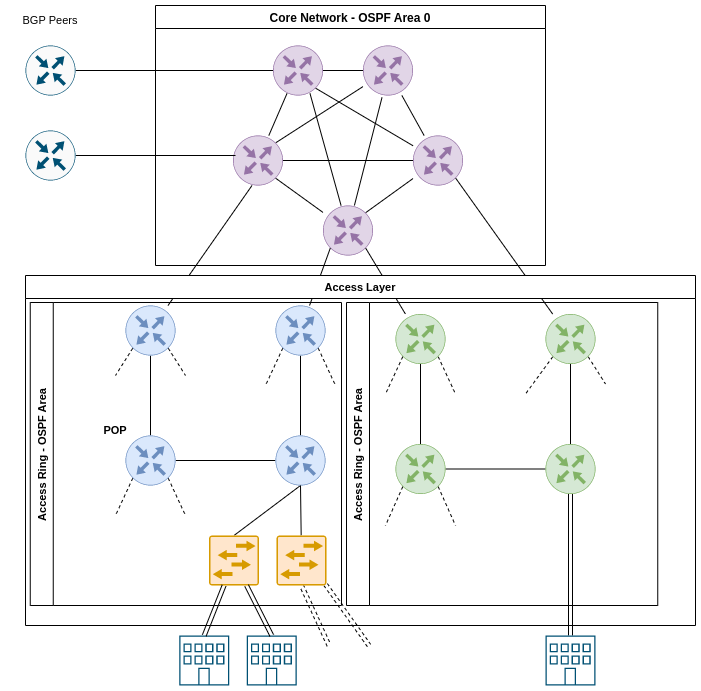
\includegraphics[width=0.7\textwidth]{Init7-Infrastructure}
  \caption{Init7 Topology}
  \label{fig:topology}
\end{figure}

This thesis is limited to the access layer, which encompasses the shown PoPs with their access switches in \ref{fig:topology}.



